\chapter{ミラー計測実験}
\thispagestyle{empty}
\label{chap5}
\graphicspath{{chap5/figure/}}
\minitoc

\newpage
%%%%%%%%%%%%%%%%%%%%%%%%%%%%%%%%%%%%%%%%%%%%%%%%%%%%%%%%%%%%%%%%%%%%%%%%%%%%%


% ================================================== %
% section
% ================================================== %
\section{諸言}
\label{chap5_introduction}

\clearpage
% ================================================== %
% section
% ================================================== %
\newpage

\section{実験の構成}

実験装置の概要を以下に示す。図\ref{fig:mirror_experiment_asm_cad_side}が横から見たcad図、図\ref{fig:mirror_experiment_asm_cad_isometric}が俯瞰して見た図である。

\begin{figure}[!ht]
\centering
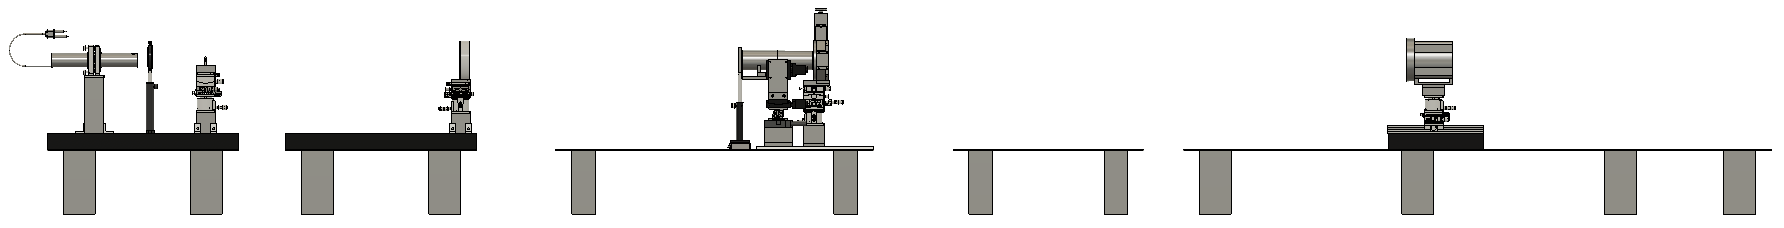
\includegraphics[width=10cm]{setup/asm_total_side.png}
\caption{ミラー測定実験系 側面図}
\label{fig:mirror_experiment_asm_cad_side}
\end{figure}

\begin{figure}[!ht]
\centering
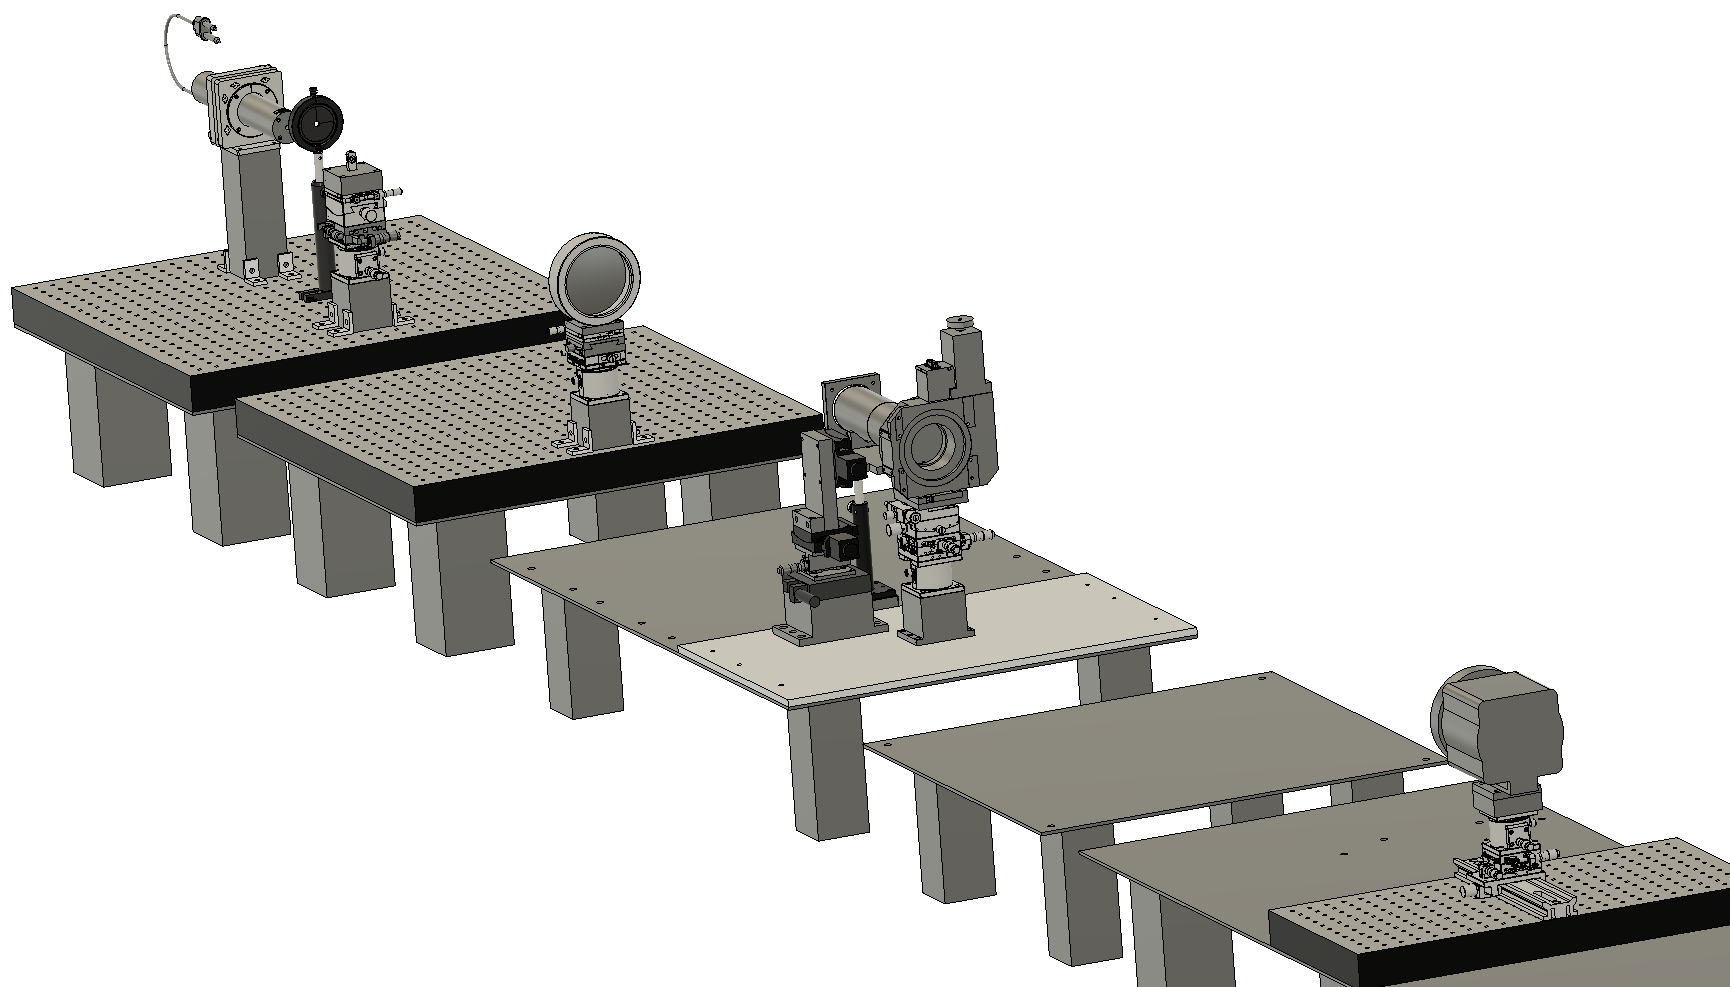
\includegraphics[width=10cm]{setup/asm_total_isometric.png}
\caption{ミラー測定実験系 俯瞰図}
\label{fig:mirror_experiment_asm_cad_isometric}
\end{figure}


\clearpage

% ================================================== %
% section
% ================================================== %
\newpage

\section{疎条件を利用した場合の結果}

\clearpage
% ================================================== %
% section
% ================================================== %
\newpage


\section{下流端走査タイコグラフィの結果}
\subsection{ピンホール1つ穴の場合}
\subsection{ピンホール2つ穴の場合}
\subsection{ピンホール3つ穴の場合}

\clearpage
% ================================================== %
% section
% ================================================== %
\newpage

\section{回復波面の解析}
\subsection{周方向誤差の真円度測定結果との比較}

% ================================================== %
% section
% ================================================== %
\section{結論}
\label{chap5_conclusion}


%%%%%%%%%%%%%%%%%%%%%%%%%%%%%%%%%%%%%%%%%%%%%%%%%%%%%%%%%%%%%%%%%%%%%%%%%%%%%

%%% Local Variables:
%%% mode: katex
%%% TeX-master: "../thesis"
%%% End:
